\chapter{Fully Automated Exploration System}
	
\section{Suggested ROS Framework} \label{rosframe}
	
	In this section a framework to test and build an entire automated system is suggested. This framework includes a 
	simulated environment, that realistically makes it possible, to navigate a drone within an simulated environment. The environment 
	is based on the Roboter Operating System (ROS).
	
	Just like our proposed system, most other automated exploration systems are based on the combination of a SLAM algorithm and 
	a path planning algorithm \cite{aut1} \cite{deep} \cite{accurat} \cite{aut2}. One example, where automated exploration with a drone is 
	applied in real life is described in the work with the title A Fully-Autonomous Aerial Robot for Search and Rescue Applications
in Indoor Environments using Learning-Based Techniques by Sampedro c. at al \cite{aut1}. They propose a complex framework targeted for search and 
    rescue operations. One issue, that becomes clear and will not be treated in our work, is the weight of the hardware, that is necessary to perform all computations 
	onboard. While the drone in Sampedro's work had to compute even more processes, such as running a constitutional neural network for object classification, 
	amounted to a total weight of 3.2 kg. Even if the drones for our purpose will not be as heavy, processing the computations onboard of an ardrone 2.0, as 
	it is used in our simulation, is impossible. When taking our proposed framework to a real life scenario, as it is also discussed in this chapter, 
	the drone would have to hold a wireless connection (WIFI in case of the ARdrone 2.0) to a server, that does all the computations. Or, another drone would have to be used, in order 
	to carry the hardware, that is needed for computation. 
	
	The basic idea of our framework can be seen in figure \ref{fig:autsys}. The main parts of the automated exploration system are the SLAM Algorithm itself
	and the flight path planning algorithm, that work simultaneously. The general concept is that each of the algorithms takes the output of the other as 
	input. 
	
	In the following section the suggested ROS framework is proposed and described in detail. 
		
	ROS stands for Roboter Operating System and as the name suggests, is a framework made to manage the software infrastructure within a robot. With the right drivers installed, 
	it can access and use the robots hardware and serves as a messenger system between robot components. ROS packages make it easy to 
	reuse important functionalities.

	Gazebo on the other hand is an open-source 3D dynamic simulator for robotics. It can accurately and efficiently simulate robots regarding
	their physics and behavior. While gazebo simulations of drones can be created from scratch, this work relies on a framework, that was introduced 
	by the robotics department of the Technische Universität München (TUM). Details can be found in section \ref{tumsec}.
	
	The suggested ROS setup consists of different nodes. Each node runs a process where certain computations are performed. These computations are based on input data
	and in most cases, the nodes also create data to output to the system. Within ROS, data is shared and received over so called rostopics (in short topics), which is a simple publish-subscribe-pattern 
	for network communication. Each node can therefore publish the computed 
	data over a certain topic or it can recieve data from a certain topic by subscribing it. The frequency, the data is streamed to the system is also defined for each 
	topic. The frequency the data is received can also be manually defined for each subscription. 
	
	\fig{img/aut_ros.png}{Overview over the suggested ROS framework for the simulated case}{fig:autros}{1}
	
	In figure \ref{fig:autros} the suggested setup for an automated exploration framework within a virtual environment is displayed. The system consists of five nodes. 
	While the functionality of the ORB-SLAM node, the TUM simulation node and the fight path planning node may be derived by previous section, such as the upper part of 
	this section and the introduction, the functionality of the other two nodes have not been introduced. 
	
	To take advantage out of the fact, that running these algorithms in a simulated environment provides the system with information about the exact position of the 
	drone and the position of simulated environment, these information must be processed. This is done in the alignment node and the transformation and restriction node. 
	
	The alignment node computes the parameters, that are needed to transform the reference frame of the ORB-SLAM algorithm to the reference frame of the gazebo simulation. 
	The actual transformation of the point cloud and the pose computed by ORB-SLAM are then performed in the transformation and restriction node. Additionally, this nodes 
	restricts the searching space of the path planning algorithm to a finite area. With the help of these two nodes, the system is then able to: 
	
	\begin{itemize}
	
	\item{Identify the true scale of the point cloud}
	\item{Confirm the correctness of the computed point cloud}
	\item{Confirm the correctness of the computed trajectory}
	\item{Limit the searching space of the path planning algorithm}
	\item{Feed the path planning algorithm with collision information of the drone}
	\item{Identify undiscovered spaces} 
	
	\end{itemize}
	
	
	\fig{img/aut_ros_real.png}{Overview over the suggested ROS framework for the real life case}{fig:autrosreal}{1}
	
	Obviously, when testing the system in a real life environment, the ground truth of the position of the environment and drone are not available. 
	Nevertheless, in order to get the true scale of the resulting point cloud, a modified framework is introduced additionally. This framework suggests an 
	initialization process, that allows for an estimation of the position of the drone. 
	
	The functionality of all nodes are described in detail in the next sections. 
	
	Since the nodes are only dependent on each other in a way that they communicate over standardized messenges, they are independent of the programming language. 
	This means that while the ORB-SLAM node is implemented in C++, all nodes developed explicitly for this framework are implemented in python with rospy. 
	
	\subsection{TUM Simulation Node} \label{tumsec}
	
	\fig{img/tum_sim.png}{Tum simulator setup. Source: http://wiki.ros.org/tum\_simulator}{fig:tumsim}{0.8}
	
	Thus, with the tum\_simulation package you can navigate an AR.drone 1.0 and 2.0 in different worlds created within gazebo. This drone is equipped with a bottom camera 
	and a front camera. The cameras each log their output to a topic. Additionally, message time stamps, the height sensor output, 
	battery percentage, rotation
	velocity and acceleration are also logged to topics. While the drone can also be navigated using a PlayStation 3 controller, as shown in figure 
	\ref{fig:tumsim}, showing a section of the tum\_simulation package content structure, 
	for an automated system, the drone should rather be addressed by publishing messages to the drone control topic (/cmd\_vel)
	using the command line interface. For example 
	by publishing messages of the class Twist, the drone can be navigated. With the command shown in listing \ref{lst:drone_cmd}, the drone is 
	controlled to fly forward, as the linear translation vector points only in the x direction.  
	
	\begin{lstlisting}[language=bash, caption= Drone navigation command, label=lst:drone_cmd]
	# navigate the drone forward
    rostopic pub -r 10 /cmd_vel geometry_msgs/Twist  '{linear:  {x: 1.0, y: 0.0, z: 0.0}, angular: {x: 0.0,y: 0.0,z: 0.0}}'
	\end{lstlisting}
	
	In the next sections, the input and output topics of the drone are discussed. 
	
	\subsubsection{Input}
	
	\begin{enumerate}
	\item{/cmd\_vel}
	
	As mentioned, the node is subscribed to the /cmd\_vel topic. Whenever a valid navigation message is received, the drone reacts accordingly, 
	if it can. 
	
	\end{enumerate}
	
	\subsubsection{Output}\label{simout}
	
	The drone has many sensors attached and more than thirty topics are logged to the system. However, here only the topics, that are of importance 
	for the automation framework will listed. 
	
	\begin{enumerate}
	
	\item{/ardrone/front/camera\_info}
	
	Over the /ardrone/front/camera\_info topic, the node publishes messages of the class CameraInfo. These messages include information about 
	image dimension, timestamp and information about the camera specific values, described in section \ref{camcalib}. In the case of the ardrone 2.0,
	the front camera generates images with 640x360 pixels and the intrinsic camera matrix is given by: 
	
	$$K = \begin{pmatrix} 374.6706070969281 & 0.0 & 320.5 \\
						  0.0 & 374.6706070969281 & 180.5 \\ 
						  0 & 0 & 1 \end{pmatrix}$$
	
	\item{/ardrone/front/image\_raw}
	
	The node publishes the actual output image data of the front camera in the /ardrone/front/image\_raw topic. The metadata of the camera are provided in the topic /ardrone/front/camera\_info described above. 
	
	\item{/ardrone/navdata}
	
	Messages of the specially developed class Navdata are published to this topic by this node. These messages include information about 
	battery percentage of the drone, state of the drone (e.g hovering, flying, init, landing...), pressure, temperature, wind, velocity and 
    some more information. These messages are also timestamped. 	
	
	\item{/ardrone/takeoff}
	
	As the name of the topic suggests, the drone takes off, when empty messenges are published to the thred. How this looks exactly can be found in 
	listing \ref{camcalib}.
	
	\item{/gazebo/model\_states}
	
	Gazebo provides the possibility to access the current pose of each model existing in a respective gazebo world. For example the ardronetestworld, 
	that is displayed in figure \ref{fig:simfigs}, consists of the drone itself, several houses, a barrier etc.
	
	Therefore, the /gazebo/model\_states topic 
	publishes the list of the pose, $x_i \in \text{SE}(3)$ of each model. However, in the ardronetestworld, only the drone is dynamic and important for this topic, all other models 
	are static and therefore the pose will not change. 
	
	\item{/gazebo/collision}
	
	It is possible to implement a contact sensor to a gazebo model.
	However, currently the implementation has not yet been successful, as described in section \ref{frameissues}. 
	
	\end{enumerate}
	
	\subsubsection{Real-life framework}

	For the real life framework, no gazebo simulation is running. Instead, a node processes the sensors of the drone within a node. The output 
	topics of the drone are then limited to the drone sensors, as displayed in figure \ref{fig:autrosreal}
	
	
	\subsection{ORB-SLAM Node}\label{orbnode}
	
	The ORB-SLAM algorithm runs in a separate node. For the vocabulary file, needed for the bag of words approach, explained in section \ref{bagofword}, the 
	standard vocabulary file provided by the authors are considered. For the virtual environment, it might be useful to provide a vocabulary file 
	generated for this particular purpose, since in the simulation generated with the tum\_simulation, edged might be of different shape, e.g particularly sharp. 
	
	The node publishes the pose $x_i \in \text{SE}(3)$ and map points computed by the ORB-SLAM Algorithm. Because the original ORB ROS implementation didn't have an option for publishing data and 
	projects, that implemented this functionality, these features had to be implemented. 
	
	\subsubsection{Input}
	
	\begin{enumerate}
	\item{/ardrone/front/image\_raw}
	
	This topic is explained in the upper section \ref{simout}.
	
	\end{enumerate}
	
    \subsubsection{Output}
	
	\begin{enumerate}
	\item{/orb/pose}
	
	This topic publishes messages of the class PoseStamped. This class includes a header, where the frame\_id and most importantly a timestamp can be provided. 
	The pose is then given by x, y, and z position coordinates and the orientation is given with quaternions coordinates, that are discussed in section \ref{pose}. 
	The topic is published at a frequency of 30 Hz. 
	
	\item{/orb/map\_points}
	
	This topic publishes messages of the class PointCloud and also runs at a frequency of 30 Hz. The class consist of a vector of points of the 
	class Point32, all having x, y, and z coordinates containing 32 bit data. 
	 

	\end{enumerate}
	
	\subsubsection{calculation}
	
	For the calculation of the pose and map points, the section \ref{orbcomp} can be referred to. 
	

	
	\subsection{Alignment node}
	
	As mentioned in section{asdfasdf} gazebo provides the true positions of all models present in the gazebo world. Most importantly, this includes 
	the pose of the drone. In order to transform the point cloud that is computed by the ORB-SLAM algorithm to the reference of the gazebo world, the estimated 
	position by ORB-SLAM and the true position are again aligned with the method of umeyama. 
	
	Therefore, this node computes the variables, that are needed for the transformation and outputs the resulting transformation matrix, translation vector and scale. 
	
	
	\subsubsection{Input}
	
	\begin{enumerate}
	\item{/ardrone/true\_position}
	
	In order to align the trajectories, the true position of the drone is needed. 
	While gazebo provides this data in the /gazebo/model\_states topic, the model 
	positions do not include a timestamp. Because a timestamp is needed for the alignment 
	in order to only align the matching positions, another node was created to add a timestamp 
	to the gazebo output positions. This node subscribes to the /gazebo/model\_states topic 
	and provides the data with a timestamp. To keep the time error, that results in reading in 
	the topic data as small as possible, 
	the node runs at an quite high frequency of 100 Hz. 
	
	Because the node is very simple only executes the task of stamping the true positions, 
	it is not listed in this chapter. 
	
	\item{/orb/pose}
	
	To align the ground truth position and the estimated position of ORB, the /orb/pose topic published 
	by the ORB node described in section \ref{adsfaf} is subscribed to by the node. 
	
	\end{enumerate}
	
	\subsubsection{Output}
	
	\begin{enumerate}
	\item{/scale}
	
	The node publishes the scale computed with the method of umeyama to  the /scale topic. 
	
	\item{/rotation\_matrix}
	
	The node publishes the rotation matrix as a flat numpy array computed with the method of umeyama to  the /rotation\_matrix topic.
	
	\item{/translation}
	
	The node publishes the scale as a flat numpy array computed with the method of umeyama to  the /translation topic.
	
	\end{enumerate}
	
	\subsubsection{Real-life framework}
	
	In case, the framework is tested in real life, because the /ardrone/true\_position topic will be unavailable, 
	the node subscribes to the /drone\_position\_init topic, published by the position estimation node instead. 
	
	\subsubsection{Computations}
	
	If all necessary nodes are up and running, the data  logged to /orb/pose at 15Hz and to /ardrone/true\_position at 50 Hz is stored at two lists. This is done at 
	a frequency of 10 Hz. Before aligning the points in the list, it is waited until 50 points are logged to each list. If only one list has reached 
	the length of 50, new elements are stacked on top, while the oldest are removed. 
	
	Then, the lists are culled in a way, that the minimum and maximum of the timestamp align. This is done in order to save unnecessary resources in the following computations.
	transformation step. Since the lists now may be of different length because they origin from topics with different logging frequency, 
	for the shorter list, for each element the element from the other list with the smallest time difference is matched. This assures that the points 
	estimated by orb and from true position are measured at the same time. 
	
	Finally, the points are aligned by using the method of Umeyama, as described in section \ref{umeyamasec} and the scale, the rotation matrix and the translation
    vector are published to the topic. 
	
	These computational steps are processed in the main callback loop of the respective file for the node. The function of the main loop is shown in listing \ref{lst:scaleup} in order 
	to provide further clarification of the computation to the reader. 
	
\begin{lstlisting}[language=python, caption=Main part of the scale estimation node, label=lst:scaleup]
def update_trans_variables(self):
	# return, if not enough points are available
	# since no scale can be computed
	if (len(self.est_pos_orb) < 50) or (len(self.true_pos) < 50):
		print("not enough data available, waiting...")
		return

	# return the scale if it already has been calculated    
	else:
		# get minimum and maximum time for each queue to figure out, 
		# how many points can be considered for alignment. This is only done once!
		min_orb = np.min([pose_oi.header.stamp.to_sec() for pose_oi in self.est_pos_orb])
		max_orb = np.max([pose_oi.header.stamp.to_sec() for pose_oi in self.est_pos_orb])

		min_true = np.min([point_oi.header.stamp.to_sec() for point_oi in self.true_pos])
		max_true = np.max([point_oi.header.stamp.to_sec() for point_oi in self.true_pos])

		thresh_min = np.max([min_orb, min_true])
		thresh_max = np.min([max_true, max_orb])

		# cut off the queues
		orb_oi = [pose_oi for pose_oi in self.est_pos_orb if pose_oi.header.stamp.to_sec() > thresh_min]
		true_oi = [pose_oi for pose_oi in self.true_pos if pose_oi.header.stamp.to_sec() > thresh_min]

		# for the shorter remaining queue, get the matching point
		if len(orb_oi) <= len(true_oi): 
			orb_oi_final = orb_oi
			true_oi_final = []
			for pose_oi in orb_oi: 
				diffs_oi = [np.abs(pose_oi.header.stamp.to_sec() - point_oi.header.stamp.to_sec()) for point_oi in true_oi]
				true_oi_final.append(true_oi[diffs_oi.index(min(diffs_oi))])

		else:
			true_oi_final = true_oi
			orb_oi_final = []
			for pose_oi in true_oi: 
				diffs_oi = [np.abs(pose_oi.header.stamp.to_sec() - point_oi.header.stamp.to_sec()) for point_oi in orb_oi]
				true_oi_final.append(true_oi[diffs_oi.index(min(diffs_oi))])

		# now do the alignment and compute the scale
		x_orb = [pose_oi.pose.position.x for pose_oi in orb_oi_final]
		y_orb = [pose_oi.pose.position.y for pose_oi in orb_oi_final]
		z_orb = [pose_oi.pose.position.z for pose_oi in orb_oi_final]

		x_true = [pose_oi.pose.position.x for pose_oi in true_oi_final]
		y_true = [pose_oi.pose.position.y for pose_oi in true_oi_final]
		z_true = [pose_oi.pose.position.z for pose_oi in true_oi_final]
		
		orb_points = np.column_stack((x_orb, y_orb, z_orb))
		true_points = np.column_stack((x_true, y_true, z_true))
		s, R, t = align_umeyama(true_points, orb_points)
		R = R.reshape([9,])

		# finally publish the computed scale, matrix and vector
		if s>0:
			self.scale_publisher.publish(Float64(s))
		if sum(np.isnan(R)) == 0:
			self.rot_publisher.publish(R)
		if sum(np.isnan(t)) == 0:
			self.trans_publisher.publish(t)
\end{lstlisting}
	
	
	\subsection{Position Estimation Node}
	
	This node is only relevant for the real life framework. there, since no groud truth is available for the position of the drone, 
	the position estimation node approximates the position of the drone based on the velocity on the drone and the latest position. ORB-SLAM, used 
	in the visual monocular mode is as mentioned not able to extract the true scale of the environment. Estimating the true position enables us 
	to also scale the computed point cloud by the ORB SLAM node to its true scale. 
	
	This method should be done in the initialization process, by 
	only doing translational movements with the drone, such as a takeoff and a short foreward movement. No rotations should be performed with the drone 
	since the drones navigation data, such as the velocity, uses the body-frame as reference frame. Thus doing rotations would result in an incorrect 
	estimation of the position. 
	
	While relying on the information about the 
	velocity of the drone, the drone needs to have inertial sensors attached. Having these IMU sensors, as the ARdrone 2.0 in the simulation does,
	also ORB SLAM would benefit from 
	accuracy, since an integration in the algorithm is implemented. However, if drone does not have these sensors attached, 
	this node can still be beneficial, since it is possible to manually publish messages to the /drone\_position\_init topic. 
	The initialization process could then be applied 
	by manually flying the drone one meter up, and one meter foreward and logging these points to the system. Then the automation process could be started.
	
	
	Folling an overview over the input, output and computational functionality of the node. 
	
	\subsubsection{Input}
	
	The node subscribes to the following topics:
	
	\begin{enumerate}
	\item{/ardrone/navdata}
	
	This topic is beeing published with the tum simulation node described in section \ref{tumsec}.
	This node only uses the velocity vectors
	$v_x \in \mathbb{R}, v_y \in \mathbb{R}, v_z \in \mathbb{R}$ given in the unit $mms^{-1}$ included in the published navdata messages. 
	
	\item{/drone\_position\_init}
	
	The drone also subscribes to the /drone\_position\_init topic, published by itself. This topic includes messages of the class PointStamped. 
	This class includes the x, y and z coordinate of the point itself, and a timestamp.  
	The node also needs the information from this topic, 
	to read in the last position and update it based on the velocity, by doing the computations explained in the following section. The x y and z 
	coordinates are transformed to meter. 
	\end{enumerate}
	
	\subsubsection{Output}
	
	The node publishes to the following topics:
	
	\begin{enumerate}
	\item{/drone\_position\_init}
	
	This topic is explained in the upper section. The updated points are published in this topic.
	
	\end{enumerate}
	
	\subsubsection{computation}
	
	As mentioned, the computation is made based on the current velocity $$v_i = \begin{pmatrix} v_{i,x} \\ v_{i,y} \\ v_{i,z} \end{pmatrix} \in \mathbb{R}^3$$ and the 
	latest position point $$x_{i-1} = \begin{pmatrix} x_{i-1,x} \\ x_{i-1,y} \\ x_{i-1, z} \end{pmatrix} \in \mathbb{R}^3$$. Also, the time difference 
	in seconds to the last point is extracted, which is easy, since all objects from the class PointStamped can be timestamped. The difference is given by 
	$\Delta t_i =  t_i - t_{i-1}$. The updated position is the yielded by
	
	$$x_{i} = x_{i-1} + \frac{\Delta t_i * v_i}{1000} $$. 
	
	Dividing by 1000 yields the unit meter. 
	
	This recursive methodology is shown in figure \ref{fig:positionfinding}
	
	\fig{img/pos_estimation.png}{Calculation method for estimation the position in the initialization process in order to find the 
	true scale.}{fig:positionfinding}{0.8}
	
	The implementation is easily deployed and the update function, that is running in the main loop can be seen in listing \ref{lst:posupdate}. 
	
	\begin{lstlisting}[language=python, caption=Main part of the position estimation node, label=lst:posupdate]
	def update_position(self):
# get velocity in x, y and z direction
x_vel = self.navdata.vz
y_vel = self.navdata.vy
z_vel = self.navdata.vz

if x_vel is not None and y_vel is not None and z_vel is not None:
	# get time difference
	curr_time = rospy.Time.now()
	time_diff = (curr_time - self.position.header.stamp).to_sec()
	
	# create the new point
	new_point = PointStamped()
	new_point.header.stamp = curr_time
	new_point.header.frame_id = "init"
	
	# update positions
	new_point.point.x = self.position.point.x + time_diff * x_vel / 1000
	new_point.point.y = self.position.point.y + time_diff * y_vel / 1000
	new_point.point.z = self.position.point.z + time_diff * z_vel / 1000
	
	# publish
	self.position_publisher.publish(new_point)
	rospy.sleep(0.1)
	\end{lstlisting}
	
	
	\subsection{Transformation and Restriction Node}
	
	This node processes the scale, rotation matrix and translation vector computed in the alignment node and transforms the ORB pose and the point cloud computed 
	by ORB SLAM into the reference frame of the gazebo world. In addition, constrains are added to the searching space of the path finding algorithm by adding 
	walls of points in the resulting point cloud of ORB. 
	
	These processes make sense for many reasons. On the one hand transforming the ORB\_SLAM output in the gazebo world creates the possibility to compare the 
	estimated position of the ORB-SLAM-Algorithm to the ground truth position as it also has been done in the evaluation of the vSLAM algorithms. While it is 
	was not yet managed to extract the ground truth point cloud of the gazebo world, as described in section \ref{frameissues}, it is technically possible, to also 
	compare the ground truth point cloud to the generated one. On the other hand, it also enables users to track the path planned by the path planning algorithm relative
	to its surrounding in the future. 
	
	The restriction of the searching space is useful, because the aim the path planning algorithm is to explore unseen areas in in the searching space. Obviously, 
	since the path planning algorithm relies exclusively on the point cloud, unseen areas are then defined as areas, where no points are available. The gazebo world, 
	displayed in figure \ref{fig:simfigs}, exceeds in unlimited space and therefore will cause the path finding algorithm to navigate in infinite space. Also the ground, sides and 
	sky of the world have no texture, and will make it impossible to find features and therefore generate points for the ORB-SLAM-Algorithm. Unfortunately, 
	as described in the issue section \ref{frameissues}, no other world is yet available. Thus, adding points to 
	limit the searching space is crucial. This is the reason why most navigation algorithm are constructed for indoor navigation.
	
	\subsubsection{Input}
	
	\begin{enumerate}
	\item{/orb/map\_points}
	
	The ORB point cloud topic, described in section \ref{orbnode} is subscribed to by the node. 
	
	\item{/orb/pose}
	
	Since also the pose is transformed in the gazebo reference frame, the /orb/pose topic is also used as input. 
	
	\end{enumerate}
	
	\subsubsection{Output}
	
	\begin{enumerate}
	\item{/pointcloud\_transformed}
	
	The node publishes data to the topic /pointcloud\_transformed with messenges of the class PointCloud. Therefore, the point cloud contains the transformed 
	point cloud of ORB SLAM and the points, that are inserted to limit the searching space of the flight path finding algorithm. 
	The exact computations are shown 
	in section below. 
	
	\item{/pose\_transformed}
	
	Also the orb pose is transfomed and published in the /pose\_transformed topic. The timestamp for the transformed pose is taken from the original pose 
	calculated by ORB, since the alignment process relies on the timestamp, when the pose was computed. 
	
	\end{enumerate}
	
	\subsubsection{computation}
	
	First, all points $p_i$ in the point cloud and the estimated positions are transformed with the rotation matrix $R$, scale $s$ and transformation vector $t$ received 
	from the above described topics. The resulting points are therefore computed by: 
	
	$$p'_i = sRp_i + t$$.
	
	Then, the restriction points are added to the point cloud.
	The ground plane of the gazebo world has a size of 100x100, but only the center is filled with objects (models). The middle of the plane 
	lies in the exact origin of the gazebo world. The goal is to restrict the search space of the path planning algorithm to the hull of a cuboid with 15m
	height, 60m length and width. The cuboid is therefore given by: 
	
	$$\Omega = \left\{(x, y, z) \in \mathbb{R} : x \in \left[-30, 30\right] \land y \in \left[-30, 30\right] \land z \in \left[-30, 30\right] \right\}$$.
	
	Then, 10000 points for each side of the hull of $\Omega$ are added to the generated point cloud by ORB, after it was transformed. This can simply been achieved 
	in three consecutively for loops. This is shown in listing \ref{lst:const} for the upper and lower restrictions. These loops are run for the sides respectively. 
	
	\begin{lstlisting}[language=python, caption= Adding upper and lower restrictions to point cloud. , label=lst:const]
	
# bottom and top 
for x_oi in np.linspace(-30, 30, 100): 
	for y_oi in np.linspace(-30, 30, 100): 
		for z_oi in [0, 15]: 
			p_out = Point32()
			p_out.x = x_oi
			p_out.y = y_oi
			p_out.z = z_oi
			pq.points.append(p_out)

	\end{lstlisting}

	Note that for the point cloud the coordinates are only stored in 32 bit to save resources, since the point cloud can contain ten thousands of data-points. In order not 
	to overload the system, the transformation node runs on a frequency of only 5Hz, which results in smooth computation. 
	
	\subsection{Flight Path Planning Node} \label{path}
	
	The fight path planning node is in charge of autonomously navigating the drone. This should be done without colliding with any obstacles. 
	On the other hand, since the goal is to explore the environment, the algorithm should always thrive to visit new areas in order to generate 
	new map points. 
	
	While the computation of this node is not yet implemented and is not part of this work, the desired input and output can be cleanly defined. 
	Also approaches currently used in for path planning approaches in active SLAM-application are described in the computation section. 
	
	\subsubsection{Input}
	
	\begin{enumerate}
	\item{/pointcloud\_transformed}
	
	This topic is explained in the upper section. 
	
	\item{/pose\_transformed}
	
	This topic is explained in the upper section.
	
	\item{/pose\_transformed}
	
	This topic is explained in the upper section.
	
	\item{/gazebo/collision}
	
	For the simulated framework, the node also may subscribe to the /gazebo/collision topic. This enables users to penalize the algorithm in the training 
	process, in case the obstacle avoidance did not succeed.
	
	
	\end{enumerate}
	
	\subsubsection{Output}
	
	\begin{enumerate}
	\item{/cmd\_vel}
	
	The node should publish navigation commands to /cmd\_vel, as shown in example \ref{lst:drone_cmd}.
	
	\end{enumerate}
	
	\subsubsection{Computation approaches}
	
	The path planning task for autonomous exploration is also related to visual servoing, which is a technique to control a robot, by 
	directly feeding it visual information. However, for most of these thechniques, the observation target has to be predefined and is also assumed 
	to always be in the field of view. 
	
	\begin{quote}
	
	In most visual servoing methods, feedback signals for the servoing
	controller are estimated by means of multiple-view geometry assuming 
	the target scene being always within the camera field of view (FOV) \cite{servo}.
	
	\end{quote}
	
	While the research in the field of automated exploration algorithms is still in its early years \cite{early} and will probably be mainly performed 
	in simulated environment in the near future \cite{deep}, some frameworks on tackling the 
	task already exist \cite{early}, \cite{deep} \cite{accurat} \cite{lopez}. 
	
	In this section, approaches, that the path flying node could be based on are explained. 
	
	\begin{quote}
	Typically, it consists of three stages [8]: (i) the identification of all possible locations
to explore (ideally infinite), (ii) the computation of the utility or reward generated by the actions that
would take the robot from its current position to each of those locations and (iii) the selection and
execution of the optimal action \cite{deep}. 
\end{quote}

A general framework for decision making processes within a certain environment was introduced with the Partially Observable Markov Decision Processes (POMDP) framework. 
	The active SLAM problem can be formally defined within this framework. 
	The POMDP framework relies on seven components \cite{thesisvandenhof}, listed below. 
	
	\begin{itemize}
	\item{Set of States $S$}
	\item{Set of Actions $A$}
	\item{Set of conditional transition probabilities $T: \mathbb{P}(s'|s, a)$}
	\item{Reward function $R : A, S \rightarrow \mathbb{R}$}
	\item{Set of beliefs $b$}
	\item{Set of observations $Z$}
	\item{Set of conditional observation probabilities $O: \mathbb{P}(z|s)$}
	\end{itemize}
	
	$S$ defines all possible states, the drone can be in. In our case, a state is defined in the oriantation of the drone, the position of the drone and the collision sensor output.
	All possible states are contained in a combination of all possible poses $SE(3)$, while the respective translational vector has to be in the cuboid $\Omega$ defined in section \ref{adsfas},  
	and all possible collision states, which is equal to $\left\{0,1\right\}$. The current state can be extracted by the subscribed topics of this node. 
	
	All possible actions are all possible control cammands, that can be published to the /cmd topic. This includes rotational and translational manovers. A possible 
	command in order to make the drone fly forewar?? can be seen in listing \ref{asdfadsf}. 
	
	The function $T$ returns the probability, a desired state $s'$ is accessed by taking an action $a$ in the state $s$. 
	
	The reward function $R$ returns a reward in the form of a real number for an action taken in a state. In our case, the reward function should be defined in a way, that actions, resulting 
	in a great amount of new observed points should be rewarded greately, while actions, that result in no new observed features or even a crash, should be given little, no or negative reward. 
	Defining a good reward function is crucial in order for the algorithm to work properly. An example reward function for our case could look like this: 
	
	$$R(a,s) = \left\{
\begin{array}{ll}
n & \textrm{for } n \textrm{ newly explored points by ORB-SLAM,\ after action a in state s} \\
-15 & \, \textrm{if tracking is lost, after action a in state s}  \\
-30 & \, \textrm{if the drone collided, after action a in state s}  \\
\end{array}
\right. $$
	
	The belief $b$ defines the probabilty for every state, that the drone actually is in this state. Therefore all probabilites should add up to one. Not all algorithms 
	require $b$ \cite{belief}.
	
	The set of observations $Z$ equals the current pose and and current map points. Finally, $O$ returns the probabilty to make an observation $z$ while being in the state $s$.
	The POMDP is looping the follwing steps: Take action based on belief state, take observations and update belief state. The goal of the POMDP framework to 
	create a policy $\pi$ that maps states into actions. This policy is optimal, when it maximizes the sum of exprected reward in the future. There are several 
	methods to find a policy, given the above components. In this paper, three of those methods are discussed. 
	

	\begin{enumerate}
	
	\item{Reinforcement learning}
	
	Unlike most other machine learning algorithm, reinforcement learning does not require training data for learning behavior. The learning mechanism is soly based 
	on the reward, that is given for an action. % quelle!
	Q-learning approaches don't need the definition of $O$ and $T$. This is why Q-learning is defined as a model-free machine learning process \cite{deep}. 
	
	Q-learning is a method of reinforcement learning. Approaches on applying it for robot navigation exist \cite{accurat}\cite{deep}\cite{lopez}. Q-learning approaches don't need the definition of $O$ and $T$.
	Instead, Q-learning defines a recursive function $Q$ that is based on the accumulated reward for a series of actions. If a drone is in a state $s$, the action $a'$ is performed, 
	that maximizes Q \cite{lopez}. 
	
	$$a' = \pi(s) = \argmax_{a} Q(s,a)$$
	
	At each iteration, the value of $Q(s,a)$ is updated with the following term: 
	
	\begin{equation}\label{update}
    \Delta Q(s,a) = \alpha(R(a,s) + 	\gamma \argmax_{a'}Q(s', a') - Q(s, a)).
	\end{equation}
	
	$\gamma$ is called the discount factor and is a value between 0 and 1 and defines, how much weight is given to the reward for steps that are further away from the current one. 
	For example, if $\gamma = 0.8$, the third term of the cummulated sum is only weihted with ${0.8}^3 = 0.512$. Thus, the more reliable the algorithm 
	and the chosen reward funktion is, the higher $\gamma$ can be chosen, and therefore the better the algorithm plans the navigation into the future. 
	
	The exact computational steps are shown in algorithm \ref{qlearn}. 
	First, the learning rate $\alpha$, and the discount function $\gamma$ have to be predefined. One possibility to find the optimal values for $\alpha$ and 
    $\gamma$ is to perform a grid search. For the grid search and for the Q-learning algorithm also an mapping function has to designed, that maps 
	the point cloud to a value that determines, how far the target exploration process has proceeded. This function could for example be examining the point clouds 
	distribution within the searching space. 
	
	Also, a number of episodes to train the models has to be defined. This is equal to the number of runs that are 
    performed until the agent, in our case the drone, gets to a terminal state. A terminal state is a state, where the agent is finished. In our case, that would 
	be equal to the state, where the drone collided, or a termination constrain has been hit when the exploration task has been successfully finished.
	This termination constrain could for example be a reached 
	threshold of the previous defined mapping function. 
	
	Then in the algorithms while loop, in each episode, the algorithm iterates, by updating the Q-table, until 
	a terminal state is reached. 
	The Q-table is a matrix, that consists of all possible actions as columns and all possible states as rows. The Q-table is updated after every action by 
	using the update rule stated in equation \ref{update}. 
	
	
	\begin{algorithm}[H]
	\KwData{Parameters: $\alpha \in (0,1], \gamma \in (0,1],$ \ Initialize Q-table with arbitrary Q-values }
	\For{episode $\leftarrow 1$ to max episode}{
	Percieve $s_t$ \;
	\While{$s_t$ not terminal}{
		select $a_t = \pi(s_t)$\;
		Take $a_t$, Get $R(a_t, s_t)$, percieve $s_{t+1}$\;
		\eIf{$s_{t+1}$ is terminal}{$Q_t \leftarrow R(a_t, s_t)$ \;}{$Q_t \leftarrow R(a_t, s_t) + \gamma \argmax_{a'}Q(s_{t+1}, a')$}
			$Q(s_t, a_t) \leftarrow (1-\alpha) Q(s_t, a_t) + \alpha Q_t $ \;
			$s_t \leftarrow s_{t+1}$ \;
	}
	}
	\caption{Q-learning algorithm. Source: \cite{deep}}\label{qlearn}
	\end{algorithm}
	
	
	In the recent years, successes were made in the applyance of deep reinforcement learning algorithms for robotic navigation and exploration \cite{deep} \cite{accurat}. 
	These approaches don't analytically compute the output of $Q$ but rather a Deep Neural Network is created in order to predict the output. 
	Since for algorithm \ref{qlearn}, in each step each action is calculated recursivly, the computation requires a lot of computational resouces. By approximating the function Q, this is avoided. 
	
	Also research has shown, that the trained models also yield good performance for environments, where they were not trained and have no a priori knowlege. 

	
	The results of \cite{deep} also shows, that the trajectory accuracy can be increased be autonomously navigating the drone. 
	\begin{quote}
	
	D3QN results are the most remarkable in the first environment, as it
outperforms the reward that a human would obtain by manually controlling the robot (approx. 350). In the
second environment both DDQN and D3QN show a good behavior. Despite DDQN have higher SR
(and mean steps, thus), the higher mean reward obtained by D3QN proves the generation of more
optimal trajectories: smoother movements and less spins. \cite{deep}
	\end{quote}
	D3QN is also a path planning algorithm based on deep reinforcement learning proposed by Wen et al in 2020 in their work Path planning for 
	active SLAM based on deep reinforcement learning under unknown environments \cite{accurat}.
	
	\item{Other approaches}
	
	Aside from the above-discussed reinforement learning methods, other approaches to tackle the path planning task exist. 
	
	Back in 2006, Leung et al published their work Active SLAM using Model Predictive Control and Attractor based Exploration \cite{ppap2}.

	In their work Active SLAM and Exploration with Particle Filters Using Kullback-Leibler Divergence \cite{ppap1}, Carlone et al suggested....
	
	\end{enumerate}
	

	
	
	\section{Current setup}
	
	In figure \cite{fig:simfigs} the simulated environment with gazebo can be found in figure a. Here, the drone (in black) is flying in front of the building. 
	The output of the front camera is shown in figure b. In figure c, the ORB-SLAM-Algorithm was applied to the output of the front camera. Green dots represent the 
	finding of a ORB-features.
	
	\begin{figure}%
    \centering
    \subfloat[\centering gazebo simulation]{{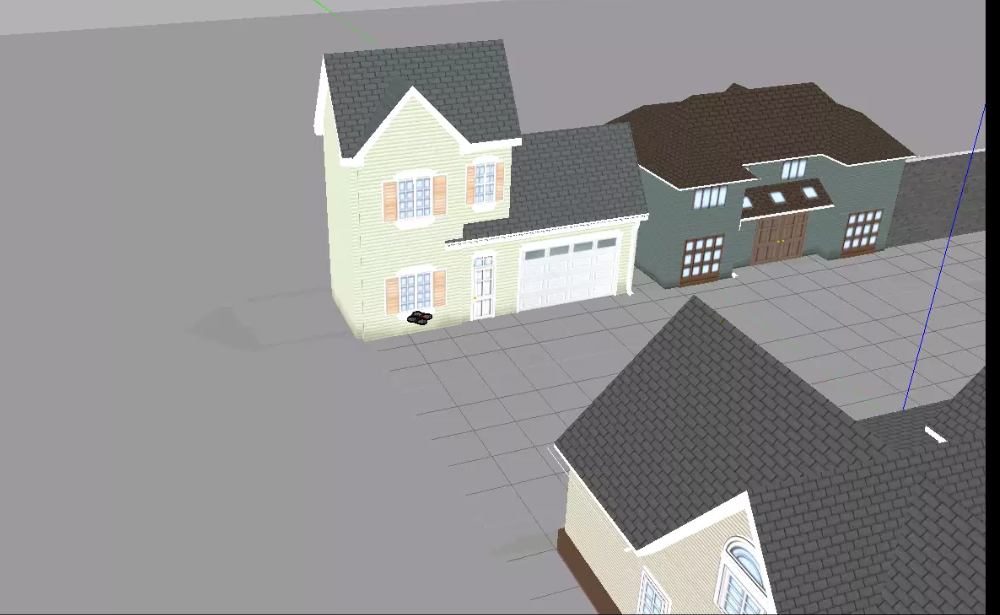
\includegraphics[width=5cm]{img/drohne_oben.png} }}%
    \qquad
    \subfloat[\centering front camera simulation]{{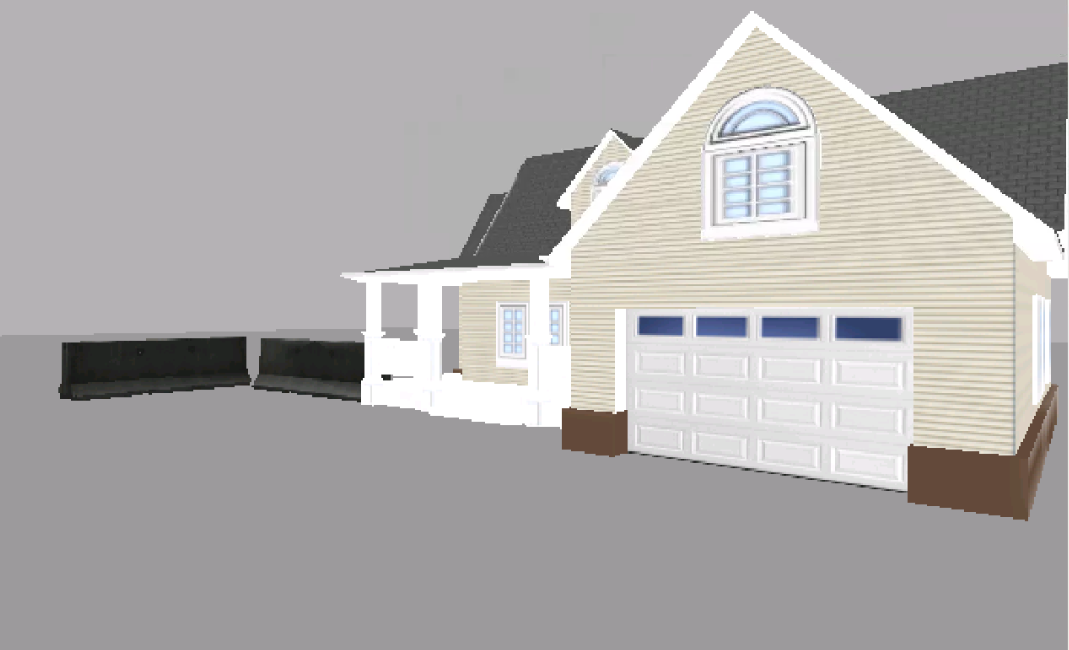
\includegraphics[width=5cm]{img/drohne_kamera.png} }}%
	\qquad
    \subfloat[\centering ORB applied on simulation]{{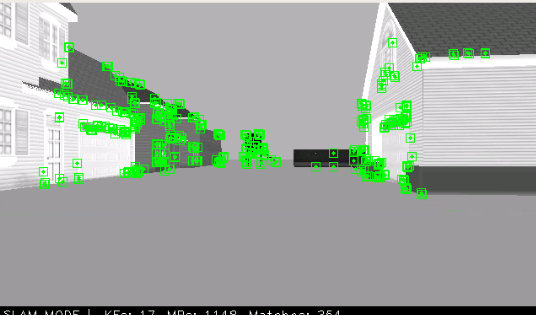
\includegraphics[width=5cm]{img/front_camera_orb.png} }}%
    \caption{
	The drone in a gazebo simulation in a), the output of the front camera of the drone in b) and
	the ORB-SLAM algorithm applied on the front camera output in with the detected ORB features marked green c).
	}%
    \label{fig:simfigs}%
	\end{figure}
	
	Currently the framework is set up in an environment provided by theconstructsim.com. This platform is enabling ROS-developers to program in preconfigured
	ROS-environments. The environment comes with the possibility to open terminal consols, a file management system, a gazebo simulator, that automatically 
	detects, when a gazebo simulation is running. Also, you have a graphical interface for other graphical applications, such as the viewer of ORB-SLAM.
	The current environments is set up with ROS kinetic and Ubuntu 16.04.6 LTS (Xenial). The tum\_simulator, ORB-SLAM and all of their dependencies are already installed. 
	The provided machine consists of 16 processing kernels and contains a total RAM space of 29 GB.  The hard drive offers 92 GB of available space. However, 
	theconstructsim.com limits each user to 8 hours daily on the platform. 
	
	The project is publicly available under the name tum simulator test.
	
	\begin{lstlisting}[language=bash, caption= Launching the simulated environment, label=lst:sim_cmd]
	
# launch the gazebo simulation
roslaunch cvg_sim_gazebo ardrone_testworld.launch
	
# launch ORB-SLAM
rosrun ORB_SLAM2 Mono ${PATH_TO_VOCABULARY} ${PATH_TO_SETTINGS_FILE}

# start the scale estimation node
rosrun auto_explorer scale_updater.py

# start the position estimation node
rosrun auto_explorer position_updater.py

# asdfasdf
# asdfasdf
	
# takeoff with drone 
rostopic pub -1 /ardrone/takeoff std_msgs/Empty

# Then start flight path planner algorithm

	\end{lstlisting}
	
	In listing \ref{lst:sim_cmd} the commands for launching the gazebo simulation, ORB-SLAM and the drone are displayed. After launching thouse 
	applications, only the path planning algorithm based on the resulting point cloud is missing. However, multiple solutions for such algorithms 
	exist \cite{path}, appying it on the system is not part of this paper and will be done in further research. 

	\subsection{Known Issues} \label{frameissues}
	
	\begin{enumerate}
	
	\item{Only one world available}
	
	For the tum\_simulator it might be useful to continue the atomation process in another simulated world. This is because the current world named ardrone\_testworld
	doesn't contain any contours or relief on the ground, and sky, as shown in figure \ref{asdfasdf}. Since the ORB-SLAM algorithm is looking for features such as edjes and changes in pixel intensites, 
	it will not find any on the ground, which will result in no points available in this are for the resulting point cloud. While there are many worlds available in the 
	tum\_simulator package, since the package is originally not made for ROS kinetic, these worlds will not compile and running the command to start one of those worlds, 
	as shown in listing \ref{lst:worldchange} will result in the follwing error: 
	
	\texttt{ERROR: cannot launch node of type [gazebo/spawn\_model]: gazebo.}
	
	So far, no solution has been detected, but one possible workaround would either to build another world from scratch. Another possible solution would be to add flying 
	constrains to the path planning algorithms, that limits the environments on a predefined volume. This solution is implemented by the bla bla node, described in section 
	\ref{dsfadf}, which restriction points to the point cloud. 
	
	
\begin{lstlisting}[language=bash, caption= Launching different world, label=lst:worldchange]
	
# launch different world named land_station1
roslaunch cvg_sim_gazebo land_station1.launch

\end{lstlisting}

	\item{No ground truth point cloud}
	
	While the pose and position of the models in the gazebo world, such as the drone itself, the houses and other objects, are known, it was not yet possible 
	to convert these objects into pointclouds. 
	
	This refuses the possibilty to compare the evaluated points by the ORB algorithm in the ROS setup, to their true position. Users of the setup now have to solely
	rely on the results of evaluation described in section \ref{asdfasdf}.
	
	\item{Collision sensor not working}

	Gazebo provides the possibility to attach collision sensors to models existing in the world. These sensors can simply be defined in the respective 
	.XML file of the model. However, even after the implementation and no error message, the respective topic, where the data should be published, 
	does not appear when calling the rostopic list cammand. So far, no solution could be found. 

	\end{enumerate}